In this strategy, mesh refinement is applied around the dominant flow features of interest.
In the current surging airfoil case, LEV is the dominant flow feature. 
Using vortex detection and tracking (see Section \ref{sec:LEV_detect_track}), LEV evolution (path and size) is determined using an initial mesh (M0\_nz25 in this case). 
Based on this a refinement zone is added around the path of the LEV.
In such a feature-based refinement, VMS-based estimated error is used to set the mesh size in the refinement zone(s) around the dominant feature(s). 
In addition, estimated error is also used to refine the mesh around the airfoil (e.g., in a similar fashion as the error-based zonal refinement discussed earlier). 
This is done to accurately resolve the flow near the airfoil including the boundary layer region that plays a direct role in the formation of LEV.

In summary, the mesh around the LEV path is refined by a factor of 2. In addition, the boundary layer mesh is refined by a factor of 2 in the streamwise direction, and again, the number of layers in the spanwise direction are doubled as compared to M0\_nz25.
The resulting mesh resolution on the surface of the airfoil in the streamwise and spanwise directions is below 40 and 25 in wall units, respectively, i.e., same as the previous cases.
This adapted mesh is referred to as the Mfa1\_nz50 mesh (where fa is short for feature-based adaptation and 1 in fa1 denotes the first iteration of mesh adaptation). 
This mesh is shown in Figure \ref{fig:FB_mesh} and the estimated error on it is shown in Figure \ref{fig:FB_error_plot}.
M0\_nz0 mesh and error field are shown again to compare against Mfa1\_nz50.
Mfa1\_nz50 contains 2,777,750 elements, which is comparable to both Mza1\_nz50 and Msa1\_nz50 meshes.

Error values are similar to those obtained on the Mza1\_nz50 mesh, i.e., near the airfoil surface, in the LEV path, and in the wake, since mesh resolution in crucial regions is similar between the Mfa1\_nz50 and Mza1\_nz50 meshes, while estimated error is higher on the Msa1\_nz50 mesh.
%Error values are lower as compared to Msa1\_nz50, since a uniform mesh size is maintained, as opposed to Msa1\_nz50, where the mesh size is patchy.
A more detailed comparison of different adaptive strategies/adapted meshes is provided in Section \ref{sec:results_adapt}.

\begin{figure}[H]
\centering
\begin{subfigure}[b]{0.475\textwidth}
\centering
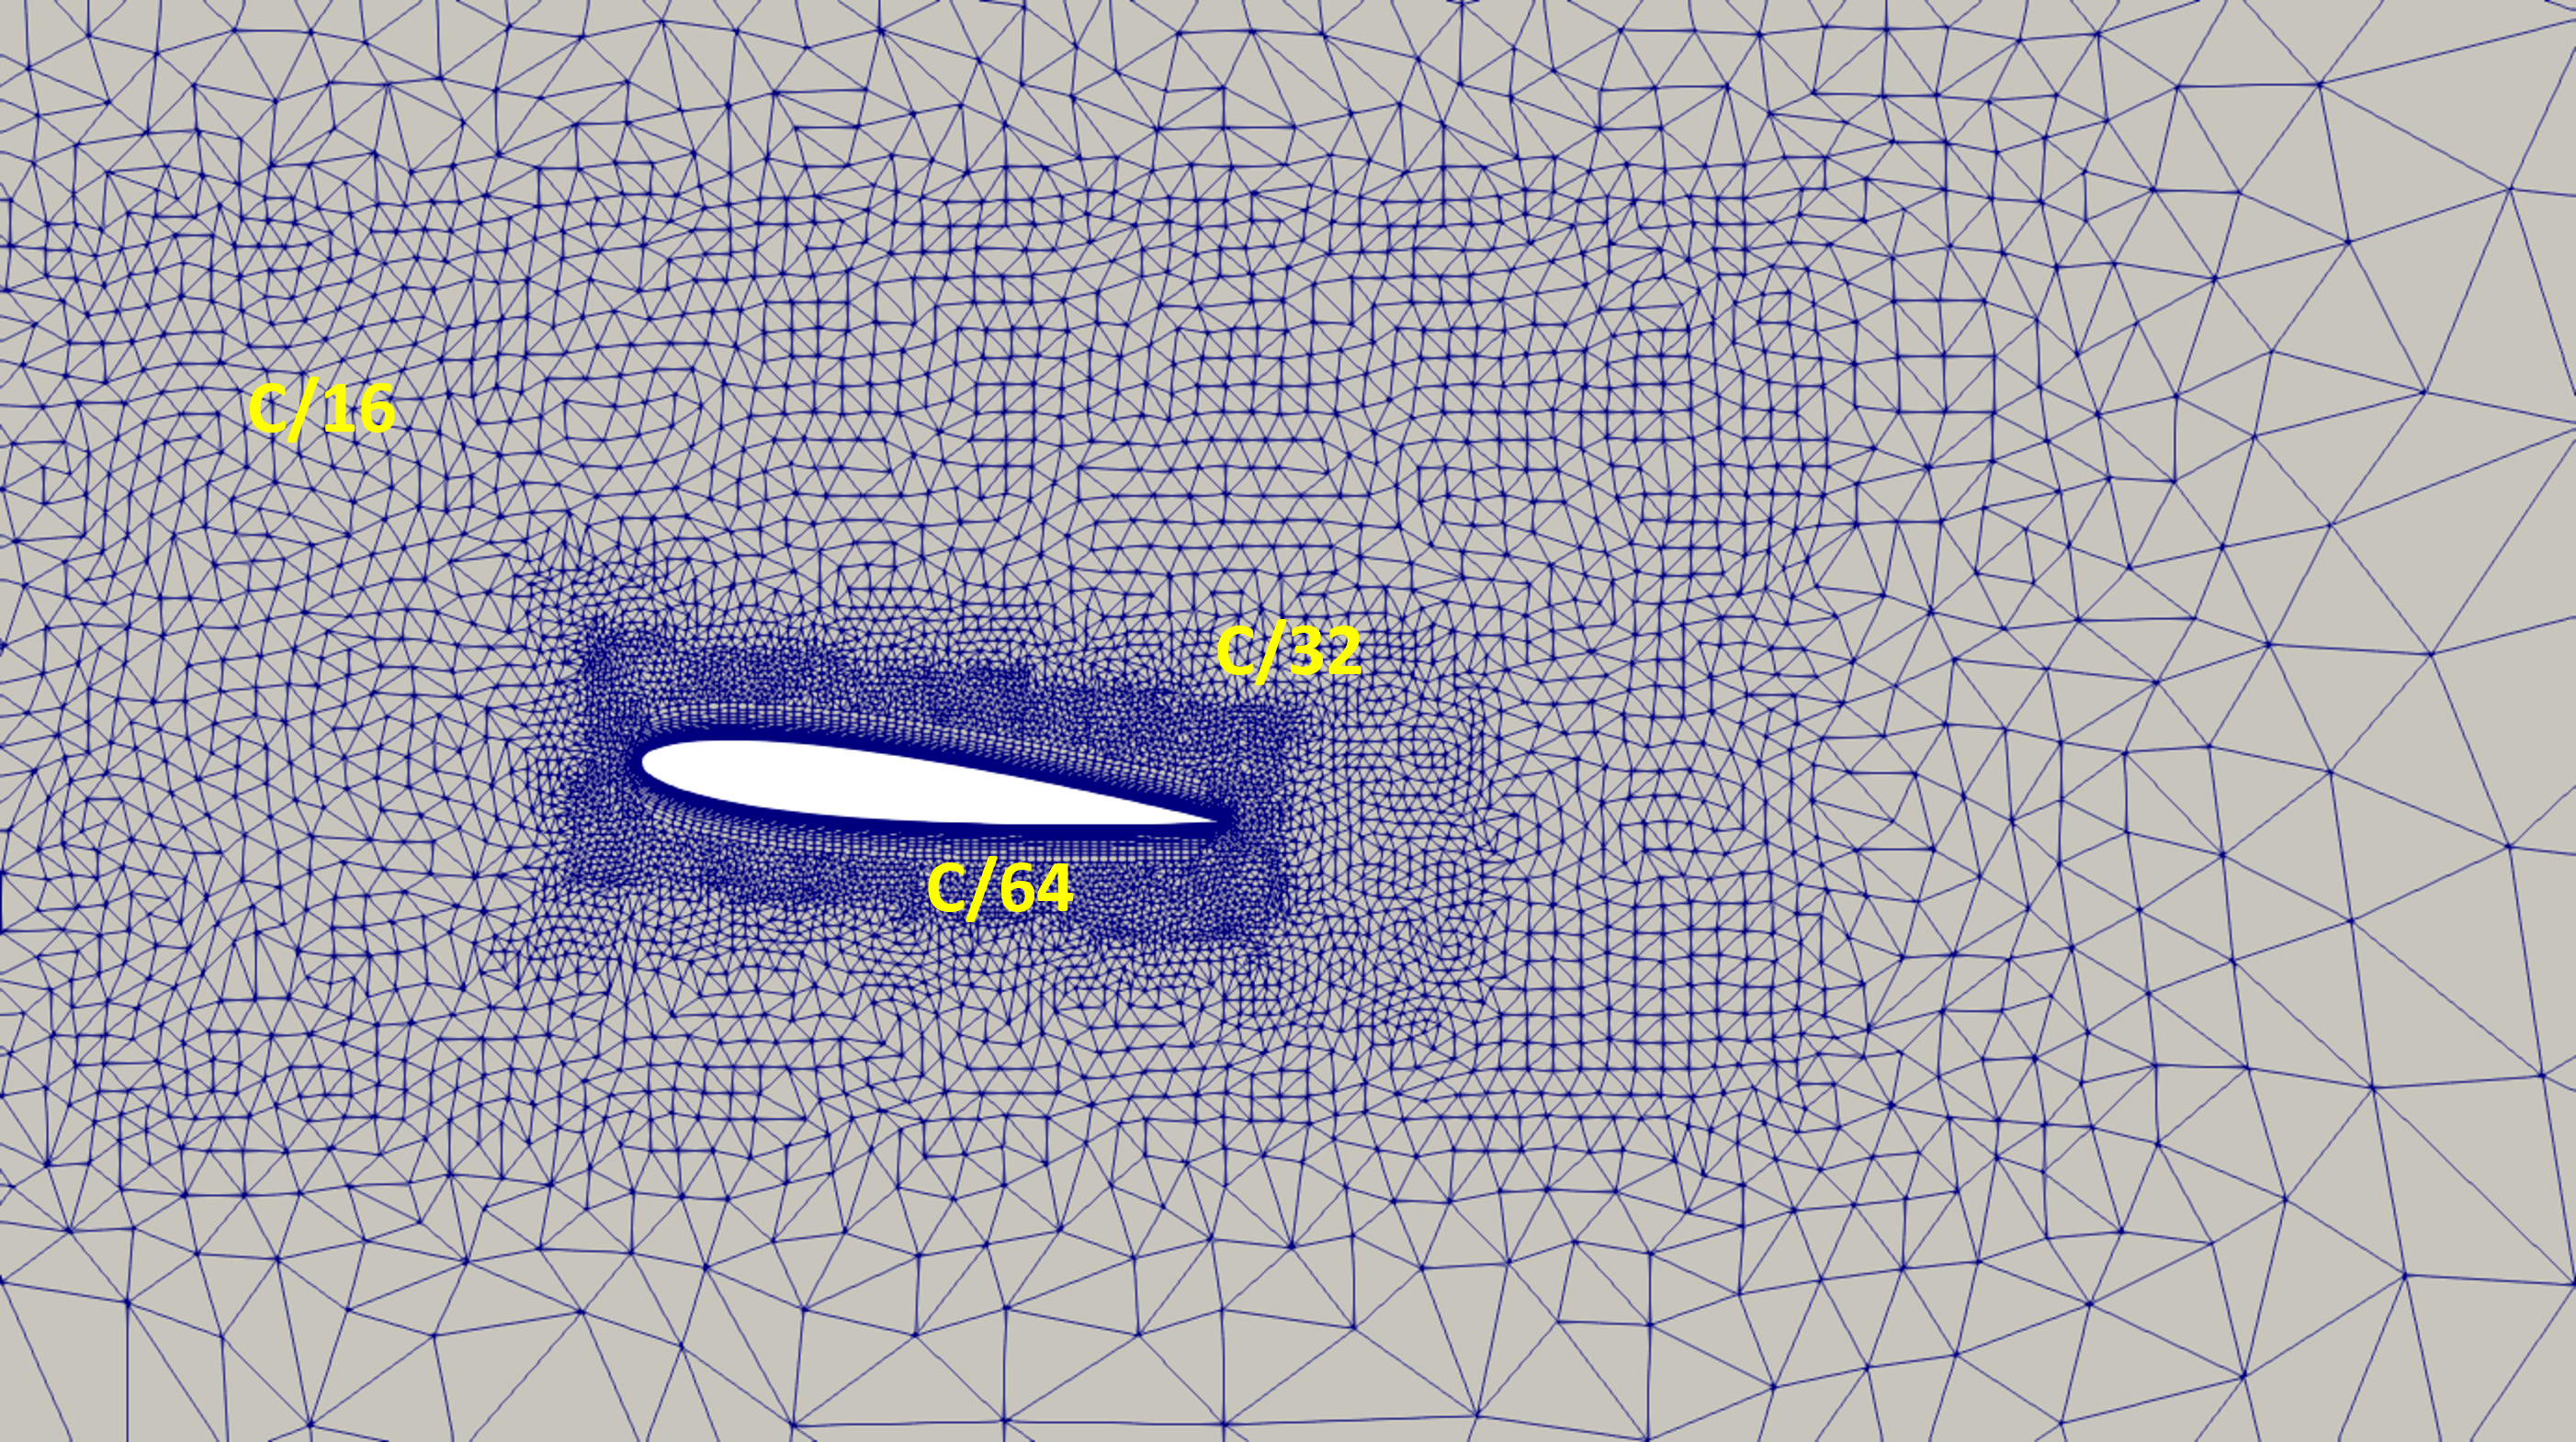
\includegraphics[width=1\textwidth]{figures/adapt_strat/M0_mesh.png}
\caption{M0\_nz25 mesh}
\label{fig:M0_mesh_fa}
\end{subfigure}
\begin{subfigure}[b]{0.475\textwidth}
\centering
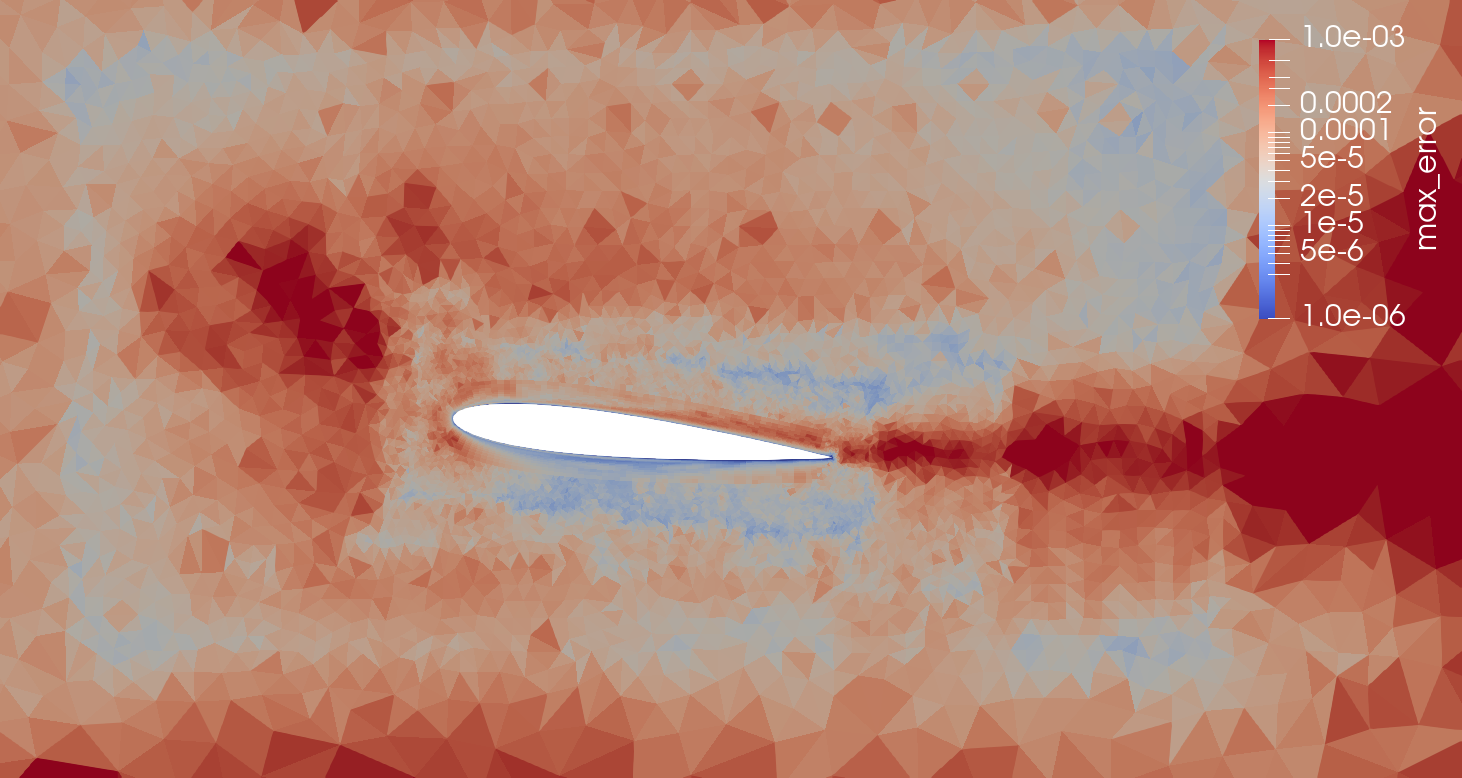
\includegraphics[width=1\textwidth]{figures/adapt_strat/M0_error.png}
\caption{M0\_nz25 error field}
\label{fig:M0_err_plot_fa}
\end{subfigure}
\begin{subfigure}[b]{0.475\textwidth}
\centering
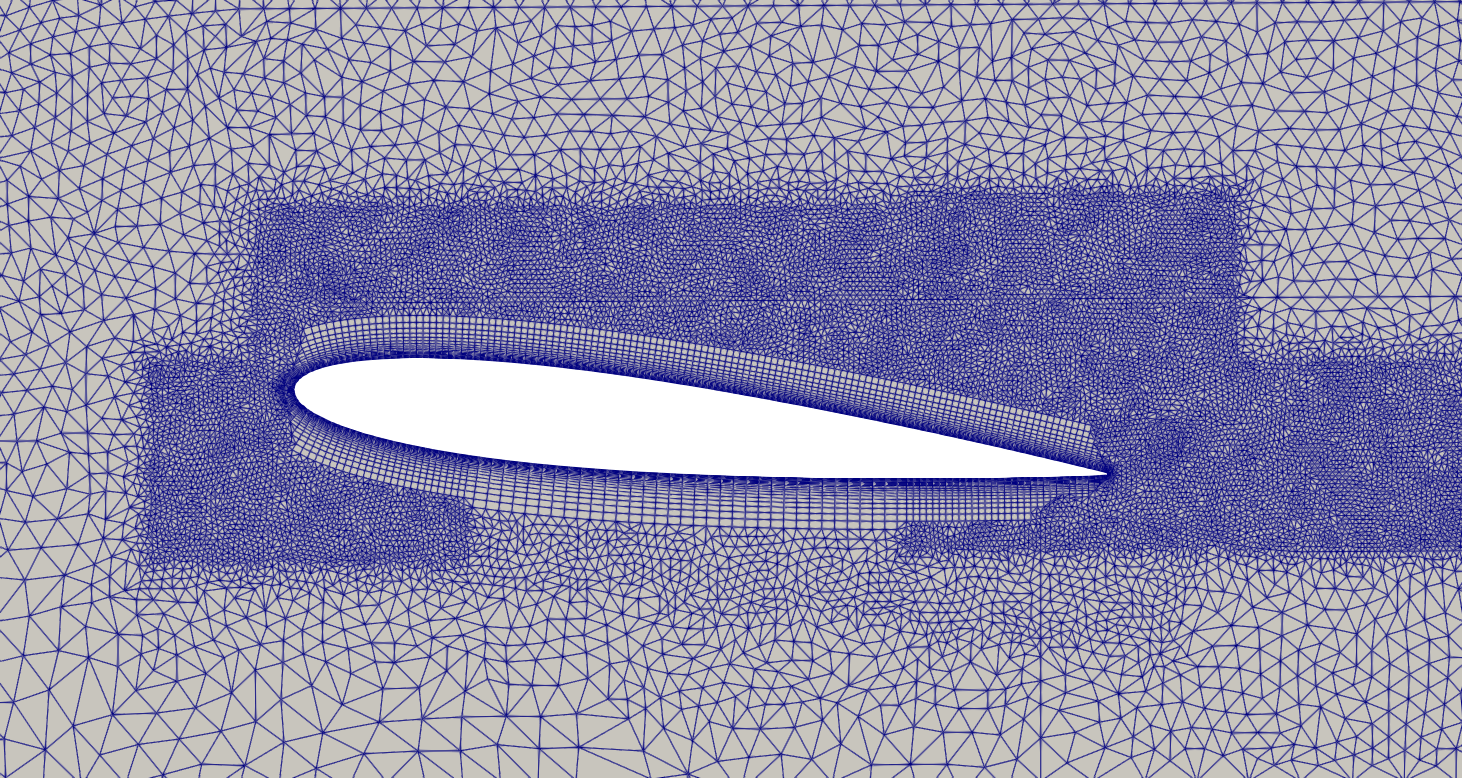
\includegraphics[width=1\textwidth]{figures/adapt_strat/Mfa1_mesh.png}
\caption{Mfa1\_nz50 mesh}
\label{fig:FB_mesh}
\end{subfigure}
\begin{subfigure}[b]{0.475\textwidth}
\centering
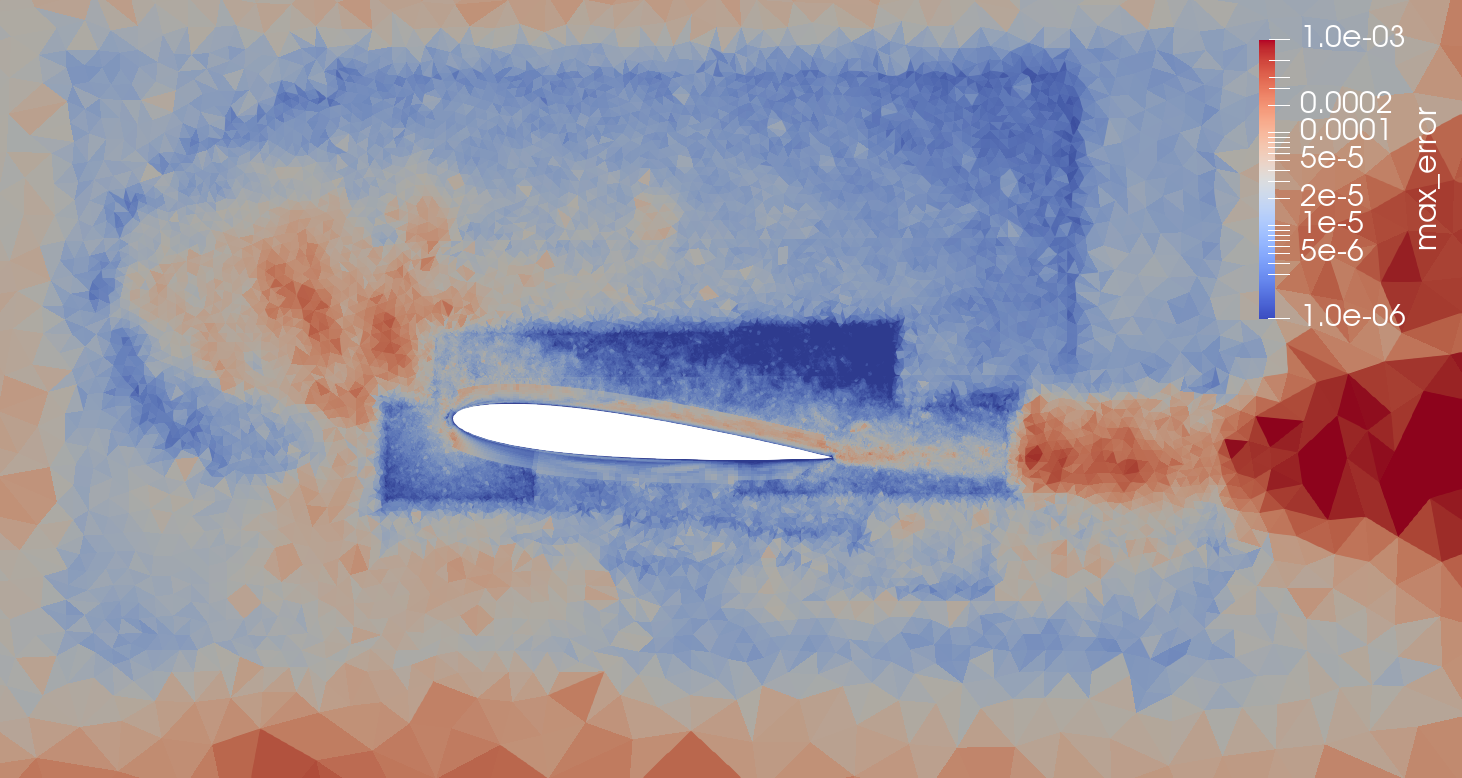
\includegraphics[width=1\textwidth]{figures/adapt_strat/Mfa1_error.png}
\caption{Mfa1\_nz50 error field}
\label{fig:FB_error_plot}
\end{subfigure}

\caption{Meshes and estimated error fields for feature-based strategy}
\end{figure}